\documentclass[11pt]{article}
\usepackage{graphicx}
\usepackage{booktabs}
\begin{document}
	\begin{titlepage}
		CS 744 Course Project
	\end{titlepage}
	\title{\textbf{\begin{huge}
			E-Commerce	
			\end{huge}}}
	\author{Debanjan Das\\
		{\small \texttt 173050069}}
	\date{\today}
	\maketitle
	\section{\label{intro}Introduction}
		Buying and selling of products online is known as \textit{e-commerce}. In this project we have created a miniature prototype of such a system. Here, multiple clients can send requests to the front-end server concurrently and front-end server should handle those requests and provide correct results to the clients.
	\section{\label{section:workpri}Working Principle}
		At first clients will run the client code in terminal window. A message will be printed, requesting the user to log-in. If user fails to log-in then program will exit. If user successfully logs in then (s)he will be shown a list of items. Out of these specified items user has to choose and order an item. The syntax of placing the order is specified in the \textit{readme.txt} file. Now, front-end server will recieve the order request and checks into it’s local database whether the item is available or not.
		\begin{enumerate}
			\item If it is \textbf{present} then it will calculate the bill and place the order and also sends request to the back-end server to update the actual database i.e,
			decrease the count of the ordered item in the actual database. Before updating front-end will check if requested count for the item is less than our capacity or not. If not then it will send an error message to client.
			Otherwise back-end server will try to update the actual database; if it succeeds then it will send positive signal to the front-end server. If it fails
			to update then it will send negative signal to front-end server. According to the response of the back-end server, front-end will take action. That is if updation succeeds then it will send client that order has been successfully placed. Otherwise it will send a failure message to the client.
			\item If the item is \textbf{not present} in the local database of front-end server then, front-end will send this request to the back-end server. Back-end will check if the item is present or not.
			\begin{itemize}
				\item If present then update in the actual database and send positive signal to the front-end server along with the bill of the user.
				\item If not present or if present but requested quantity is greater than our capacity then send a negative signal to the front-end.
			\end{itemize}
			According to the response from the back-end server, front-end will send message to the client.
		\end{enumerate}
	\section{\label{section:sysarch}System Architecture}
		\begin{figure}[h]
			\begin{center}
				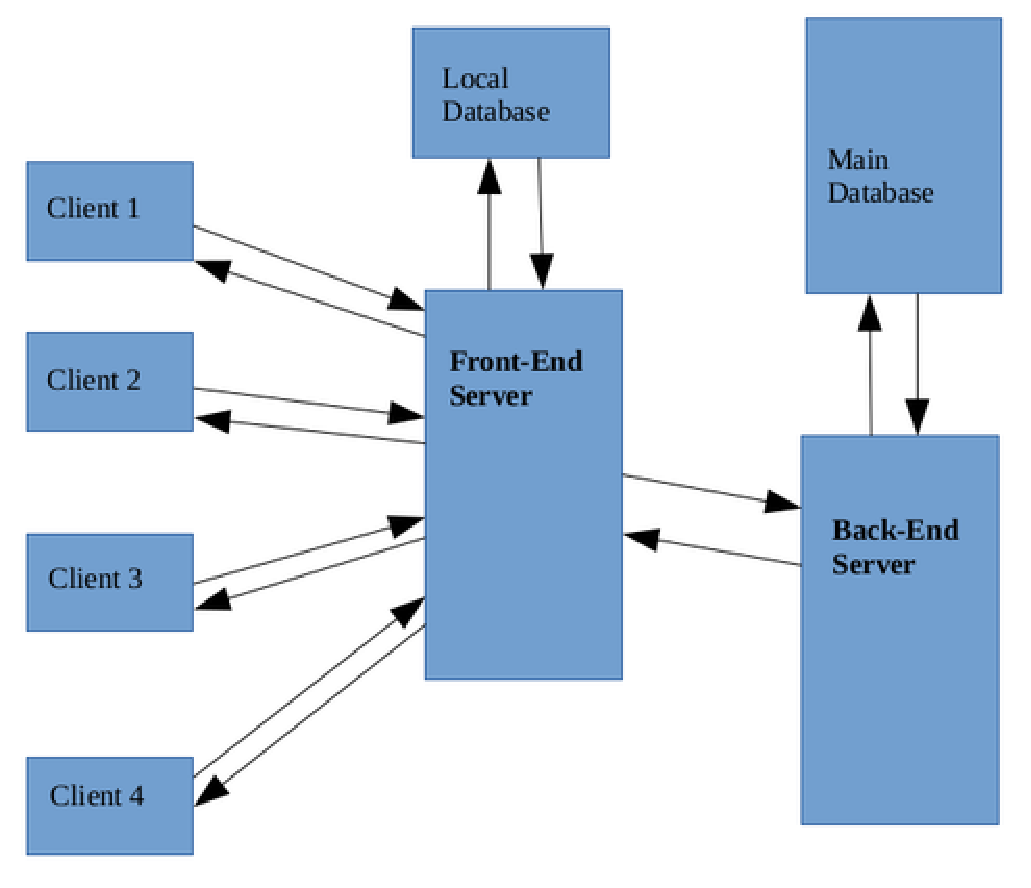
\includegraphics[scale=0.5]{block_diagram.pdf}
				\caption{\label{fig:architecture} Block Diagram of the System}
			\end{center}
		\end{figure}
		\subsection{Client}
			It has two functionalities.
			\subsubsection{log\_in()}
				Here it is taking username and password as input and
				sending them to the front-end server for authentication of client. If log in successful then it will return 1, otherwise 0.
			\subsubsection{place\_order()}
				If log in was successful then only this funtion
				will be executed. It will show all the available items to the user. And also takes order from user and sends it to the front-end server.
		\subsection{Front-End Server}
			It is multi-threaded server based on master-worker thread
			model. It can handle multiple requests at a time by assigning each worker thread to each client. And it also connects with the back-end server as a client. Then according to the user’s requests it will communicate with the back-end server. It has mainly two functionalities.
			\subsubsection{authentication()}
				Here it takes username and password from client and checks if it matches with the stored usernames and the corresponding passwords. If authentication succeeds then it will return 1, otherwise returns 0.
			\subsubsection{get\_order()}
				If authentication is successful then only this function will be executed. Here it gets the order requests from the client and processes it. First it will checks if the item is present or not. If it is present then it will calculate the bill and sends the bill and a success message to the client and also sends request to the back- end server to update the actual database i.e, decrease the count of the ordered item in the actual database. Before updating,this function will check if requested count for the item is less than our capacity or not. If not less then it will send an error message to client. Otherwise back-end server will try to update the actual database; if it succeeds then it will send positive signal to this function. If it fails to update then it will send negative signal to it. According to the response of the back-end server, this function will take action. That is if updation succeeds then it will send client that order has been successfully placed. Otherwise it will send a failure message to the client.
				
				If the item is not present in the local database of front-end server then, this function will send this request to the back-end server. Back-end will check if the item is present or not. If present then update in the actual database and send positive signal to it
				along with the bill of the user. If not present or if present but requested quantity is greater than our capacity then send a negative signal to this function. According to the response from the back-end server, it will send message to the client.
		\subsection{Back-End Server}
			It gets request from the front-end server. It gets item-name and item-count from the front-end server. Now it checks for the desired item-name into sqlite database named Products.db file. If the item is not present in the
			database then it sends a message “ This item is not present in our store” to the front-end server and if the item is present in the database then it retrives current count of the item available and price of item from the
			database. After that it compares the current count of item with the number of item front-end has requests for. If current count of item is not sufficient then it sends a message “We have only current count number of item present” to the front-end server. If it has sufficient number of item present then it updates the count of item by decrementing the current count by the number of item it has got request for and sends the total price of the purchased item to the front-end server.
		\subsection{Database}
			In case of front-end server we have used the heap memory of the front-end server program as storage of our local database. And in case of back-end server we have used SQLite database as our main database.
	\section{\label{section:performance}Performance Analysis}
		For performance analysis of the system we perform closed loop test on the system. Let us define the closed loop system.
		\subsection{Closed Loop System}
			Consider a closed loop system with N users. That is, multiprogramming level(MPL) = N. Each user submits a request, gets a response, thinks for a certain time Z, and makes another request. Total turnaround time for a request is response time at server, and think time. 
			$$E[T] = E[R] + E[Z]$$
			
			Let us now compute the ideal number of users to saturate a closed system. Assume that the closed system has many subcomponents, each with individual service demands $D_i$. The slowest component, or the bottleneck component, has service demand $D_{max}$. $D = sum(D_i)$, and $D_{max}$ is one of the $D_i$.
			
			Now, if only one user, the bottleneck component is busy for $D_{max}$ in a total time period of $D+E[Z]$. So, intuitively, $$N^* = \frac{D+E[Z]}{D_{max}}$$ number of users will keep the bottleneck fully occupied, and will lead to full utilization.
			
			\paragraph{Little's Law for Closed System:}
				Throughput increases almost linearly when N initially. But as queueing delays start to build up, throughput flattens out. Response time is almost constant initially, but increases as N increases and queues build up.
				$$N = X*E[T]$$  $$E[T] = \frac{N}{X}$$
				$$X = \frac{N}{E[R] + E[Z]}$$ 
				One of the most amazing integration formula is given as:
				$$ \int \tan^n(x)dx = \frac{1}{n-1}\tan^{n-1}(x)+\int \tan^{n-2}(x)dx  $$
				
				\begin{large}
					Shrodinger Equation is given as:
				\end{large}
				$$ \frac{\partial^2 \Psi}{\partial x^2}+\frac{8\pi^2m}{h^2}(E-V)\Psi = 0$$
				\begin{Large}
					Einstein Field Equation is given as:
					$$ R_{\mu\nu}-\frac{1}{2}Rg_{\mu\nu}+\Lambda g_{\mu\nu} = \frac{8\pi G}{c^4}T_{\mu\nu} $$
				\end{Large}
				
			\subsubsection{Generated Data}
				The table below gives the data we generated during our closed loop load testing.
				\\
				\\
				\label{table:tab1}\begin{tabular}{lrr}
\toprule
{} &  Arrival Rate(req/sec) &  Response Time & Throughput\\
\midrule
0  &            10 &            1.0 &		   \\
1  &            20 &            1.0 \\
2  &            30 &            1.0 \\
3  &            40 &            1.0 \\
4  &            50 &            1.0 \\
5  &            60 &            1.0 \\
6  &            70 &            1.0 \\
7  &            80 &            2.0 \\
8  &            90 &            4.0 \\
9  &           100 &            4.5 \\
10 &           150 &            5.0 \\
11 &           200 &            8.0 \\
12 &           250 &           16.0 \\
13 &           300 &           32.0 \\
14 &           400 &           64.0 \\
15 &           500 &          128.0 \\
16 &           600 &          256.0 \\
17 &           700 &          512.0 \\
18 &           800 &         1024.0 \\
19 &          1000 &         2048.0 \\
\bottomrule
\end{tabular}
 
				\\
				\\
				\\
				\\
				\\
				\\
				\\
				\\
				\\
				\\
			\subsubsection{Necessary Plots}
				These are some of the necessary plottings that we got from our closed loop test on our system.
				\begin{figure}[h]
					\begin{center}
						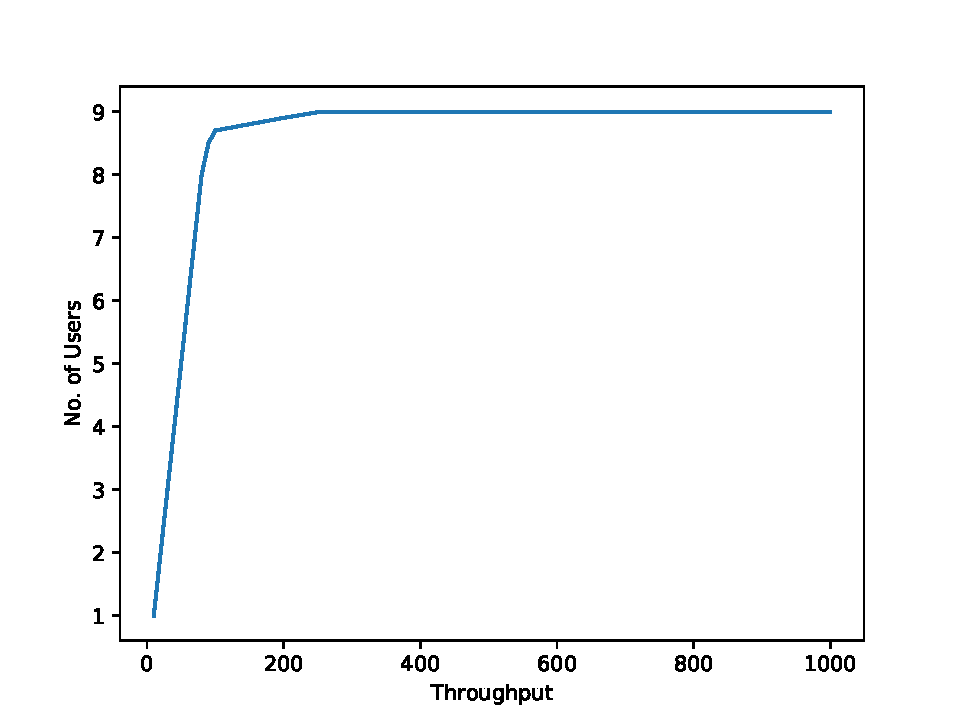
\includegraphics[scale=0.5]{plot1.pdf}
						\caption{\label{fig:plot1} Throughput vs. No.of Users}
					\end{center}
				\end{figure}		
				\begin{figure*}[ht]
					\begin{center}
						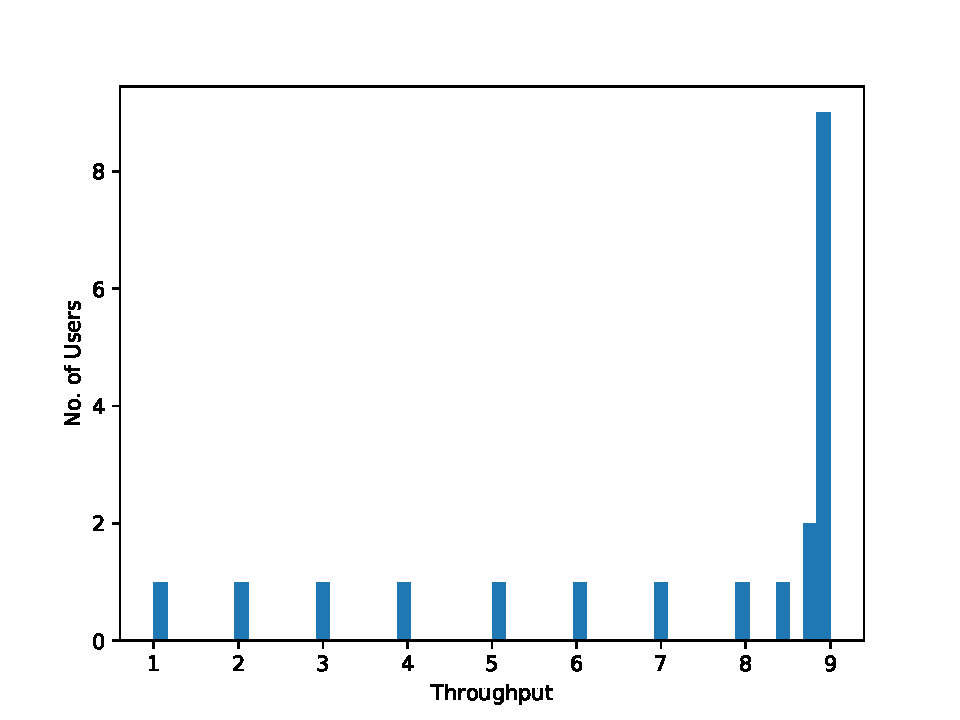
\includegraphics[scale=0.5]{plot2.pdf}
						\caption{\label{fig:plot2} Histogram of Throughput vs. No.of Users}
					\end{center}
				\end{figure*}
				\begin{figure}[ht]
					\begin{center}
						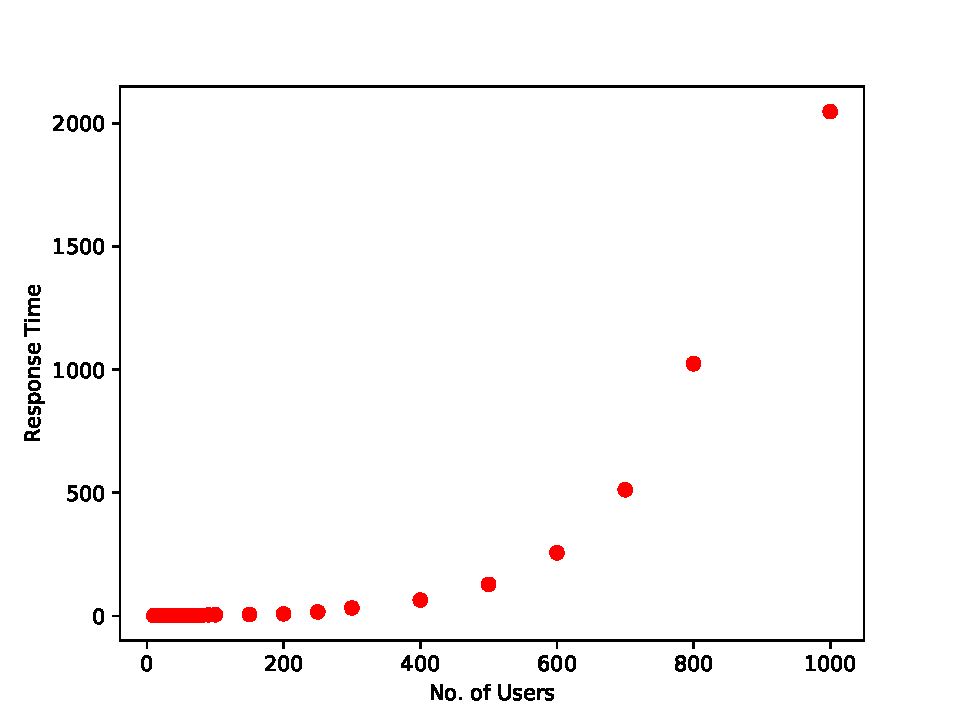
\includegraphics[scale=0.5]{plot3.pdf}
						\caption{\label{fig:plot3} Response Time vs. No.of Users}
					\end{center}
				\end{figure}
				\begin{figure}[ht]
					\begin{center}
						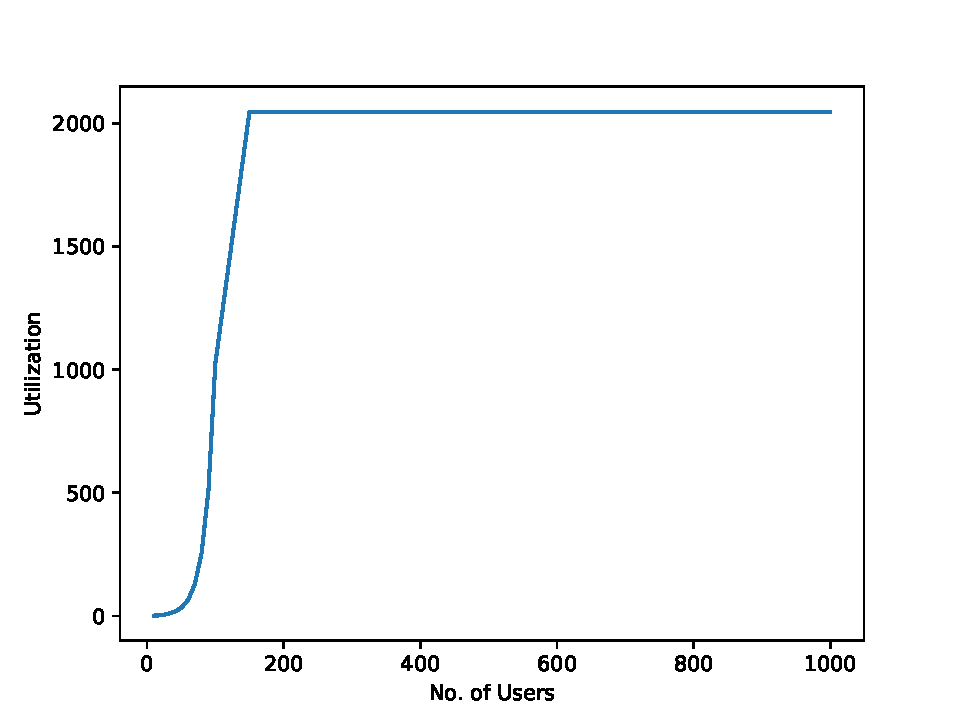
\includegraphics[scale=0.5]{plot4.pdf}
						\caption{\label{fig:plot4} Utilization vs. No.of Users}
					\end{center}
				\end{figure}
				\begin{figure}[ht]
					\begin{center}
						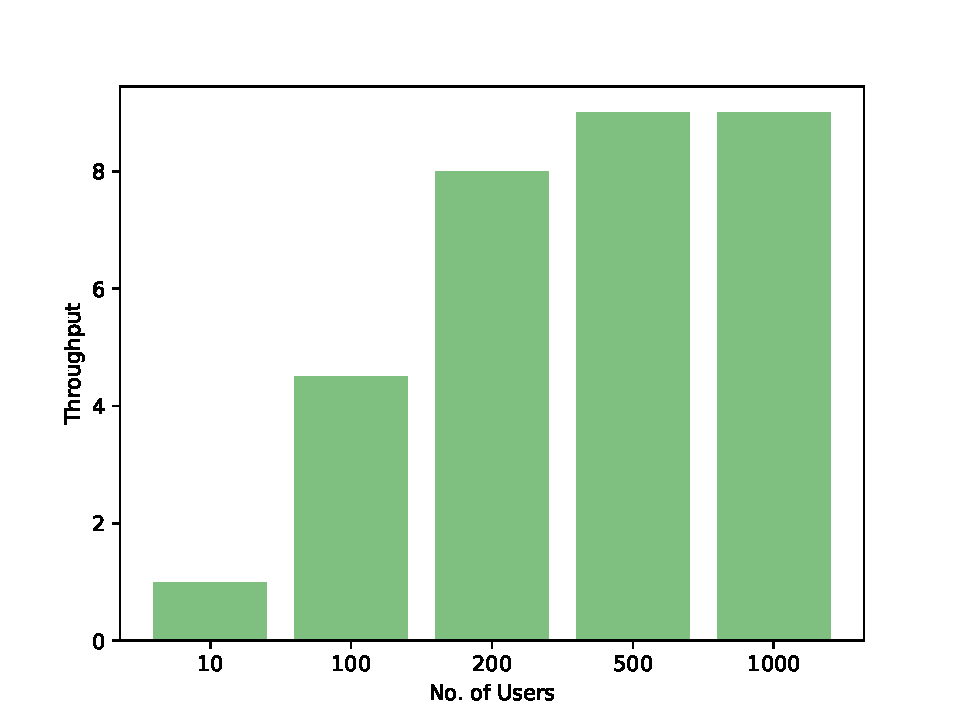
\includegraphics[scale=0.5]{plot5.pdf}
						\caption{\label{fig:plot5} Bar Chart of Throughput vs. No.of Users}
					\end{center}
				\end{figure}
	
	\clearpage							
	\section{Conclusion}
		In phase-I this system is working fine with multiple client requests and
		also updates both the databases correctly. It handles requests on first come first
		server basis. In addition to this we have also implemented successfully an
		authentication system for the users.
		
		The project is in phase-I. So we can do many improvements to this
		system, like we can build a better UI for client and we have to handle many
		corner cases e.g, if the input is not in the given format then what to do etc. In
		the next phase we are also planning to add an option to register for the clients
		and store their credentials on a seperate database at the front-end.
\end{document}